\documentclass[12pt,a4paper,oneside]{erdc}
%\documentclass{erdc}
\usepackage[T1]{fontenc}		% Selecao de codigos de fonte.
\usepackage[utf8]{inputenc}		% Codificacao do documento (conversão automática dos acentos)
%\usepackage{lastpage}			% Usado pela Ficha catalográfica
\usepackage{indentfirst}		% Indenta o primeiro parágrafo de cada seção.
\usepackage{color}				% Controle das cores
\usepackage{graphicx}			% Inclusão de gráficos
%\usepackage{microtype} 			% para melhorias de justificação
\usepackage[brazil]{babel}
%\usepackage[brazilian,hyperpageref]{backref}	 % Paginas com as citações na bibl
%\usepackage[alf]{abntex2cite}	% Citações padrão ABNT
\usepackage{hyperref}
\usepackage{natbib}

\usepackage{lipsum}


\begin{document}

\frontmatter

\laboratory{PPGE-UFPA}

\reportnum{BP/EcoS - RP-001-00-2019}

\program{Construção de Modelos e Indicadores Econômicos}

\title{PPGE-UFPA \\ Banpará}

%\subtitle{Assessments and Report from Socioeconomic and Demographic Data in \\
%	      Small Cities in Amazon Delta}

\subtitle{Relatório Parcial}

\date{\today}

\author{S.~Rivero \and H.~Farias}

\affiliation{Programa de Pós-Graduação em Economia\\
  Instituto de Ciências Sociais Aplicadas\\
  Universidade Federal do Pará\\
  Rua Augusto Correia, 1\\
  Belém, Pará - 66.075-200}

\author{L ~Silva }


\affiliation{Faculdade de Economia \\
	Instituto de Ciências Sociais Aplicadas\\
	Universidade Federal do Pará\\
	Rua Augusto Correia, 1\\
	Belém, Pará - 66.075-200}


\coverart{../figs/Abaetetuba_Rio}

\reporttype{Produto 1}

\distribution{Propriedade BANPARÁ e PPGE-UFPA \\ (Distribuição Restrita)}

% \distribution{Distribution authorized to U.S. Government Agencies
% only; Test and Evaluation; November 2005.  Other requests should be
% referred to U.S. Army Engineer Research and Development Center}

%\additionalinfo{Supersedes ERDC/CREL AF-01-23}

\begin{abstract}
  \lipsum[12-13]
\end{abstract}

\disclaimer{
	
	This document is an output from the  Banpará Project 
	
	PPGE-UFPA report
	
	Distribution Restrictions
	
	\copyright 2019, All rights reserved
	
	\pagebreak
	
	}

\preparedfor{Banpará} 

\contractnum{FADESP-NO-CONTRATO}

\monitoredby{Banpará}

%\preparedfor{}




\maketitle

\tableofcontents


\chapter*{Resumo Executivo}

  \lipsum[12-13]

\mainmatter


\chapter{Contextualização: Variáveis e Elementos Gerais}
		

  \lipsum[12-13]
   \cite{DeLima2018}	
	  		
\begin{figure}
\centering
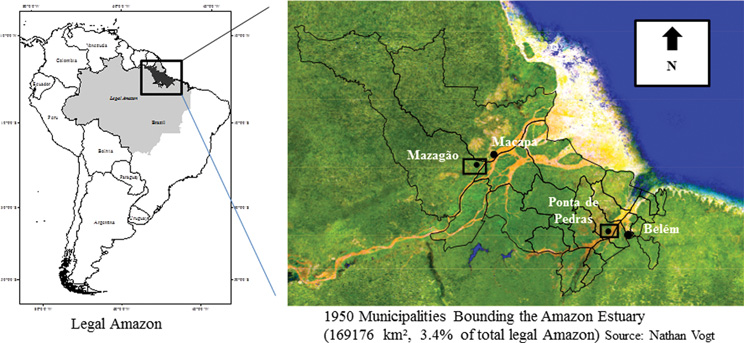
\includegraphics[width=\linewidth]{../figs/VogtEtAl2015}
\caption{O Delta Amazônico}
\label{fig:vogtetal2015}
\end{figure}

  \lipsum[12-13]
  
  
\section{Variáveis}

  \lipsum[12-13]



\chapter{Metodologia}

  \lipsum[12-13]

\section{Calibração}

\begin{figure}
	\centering
	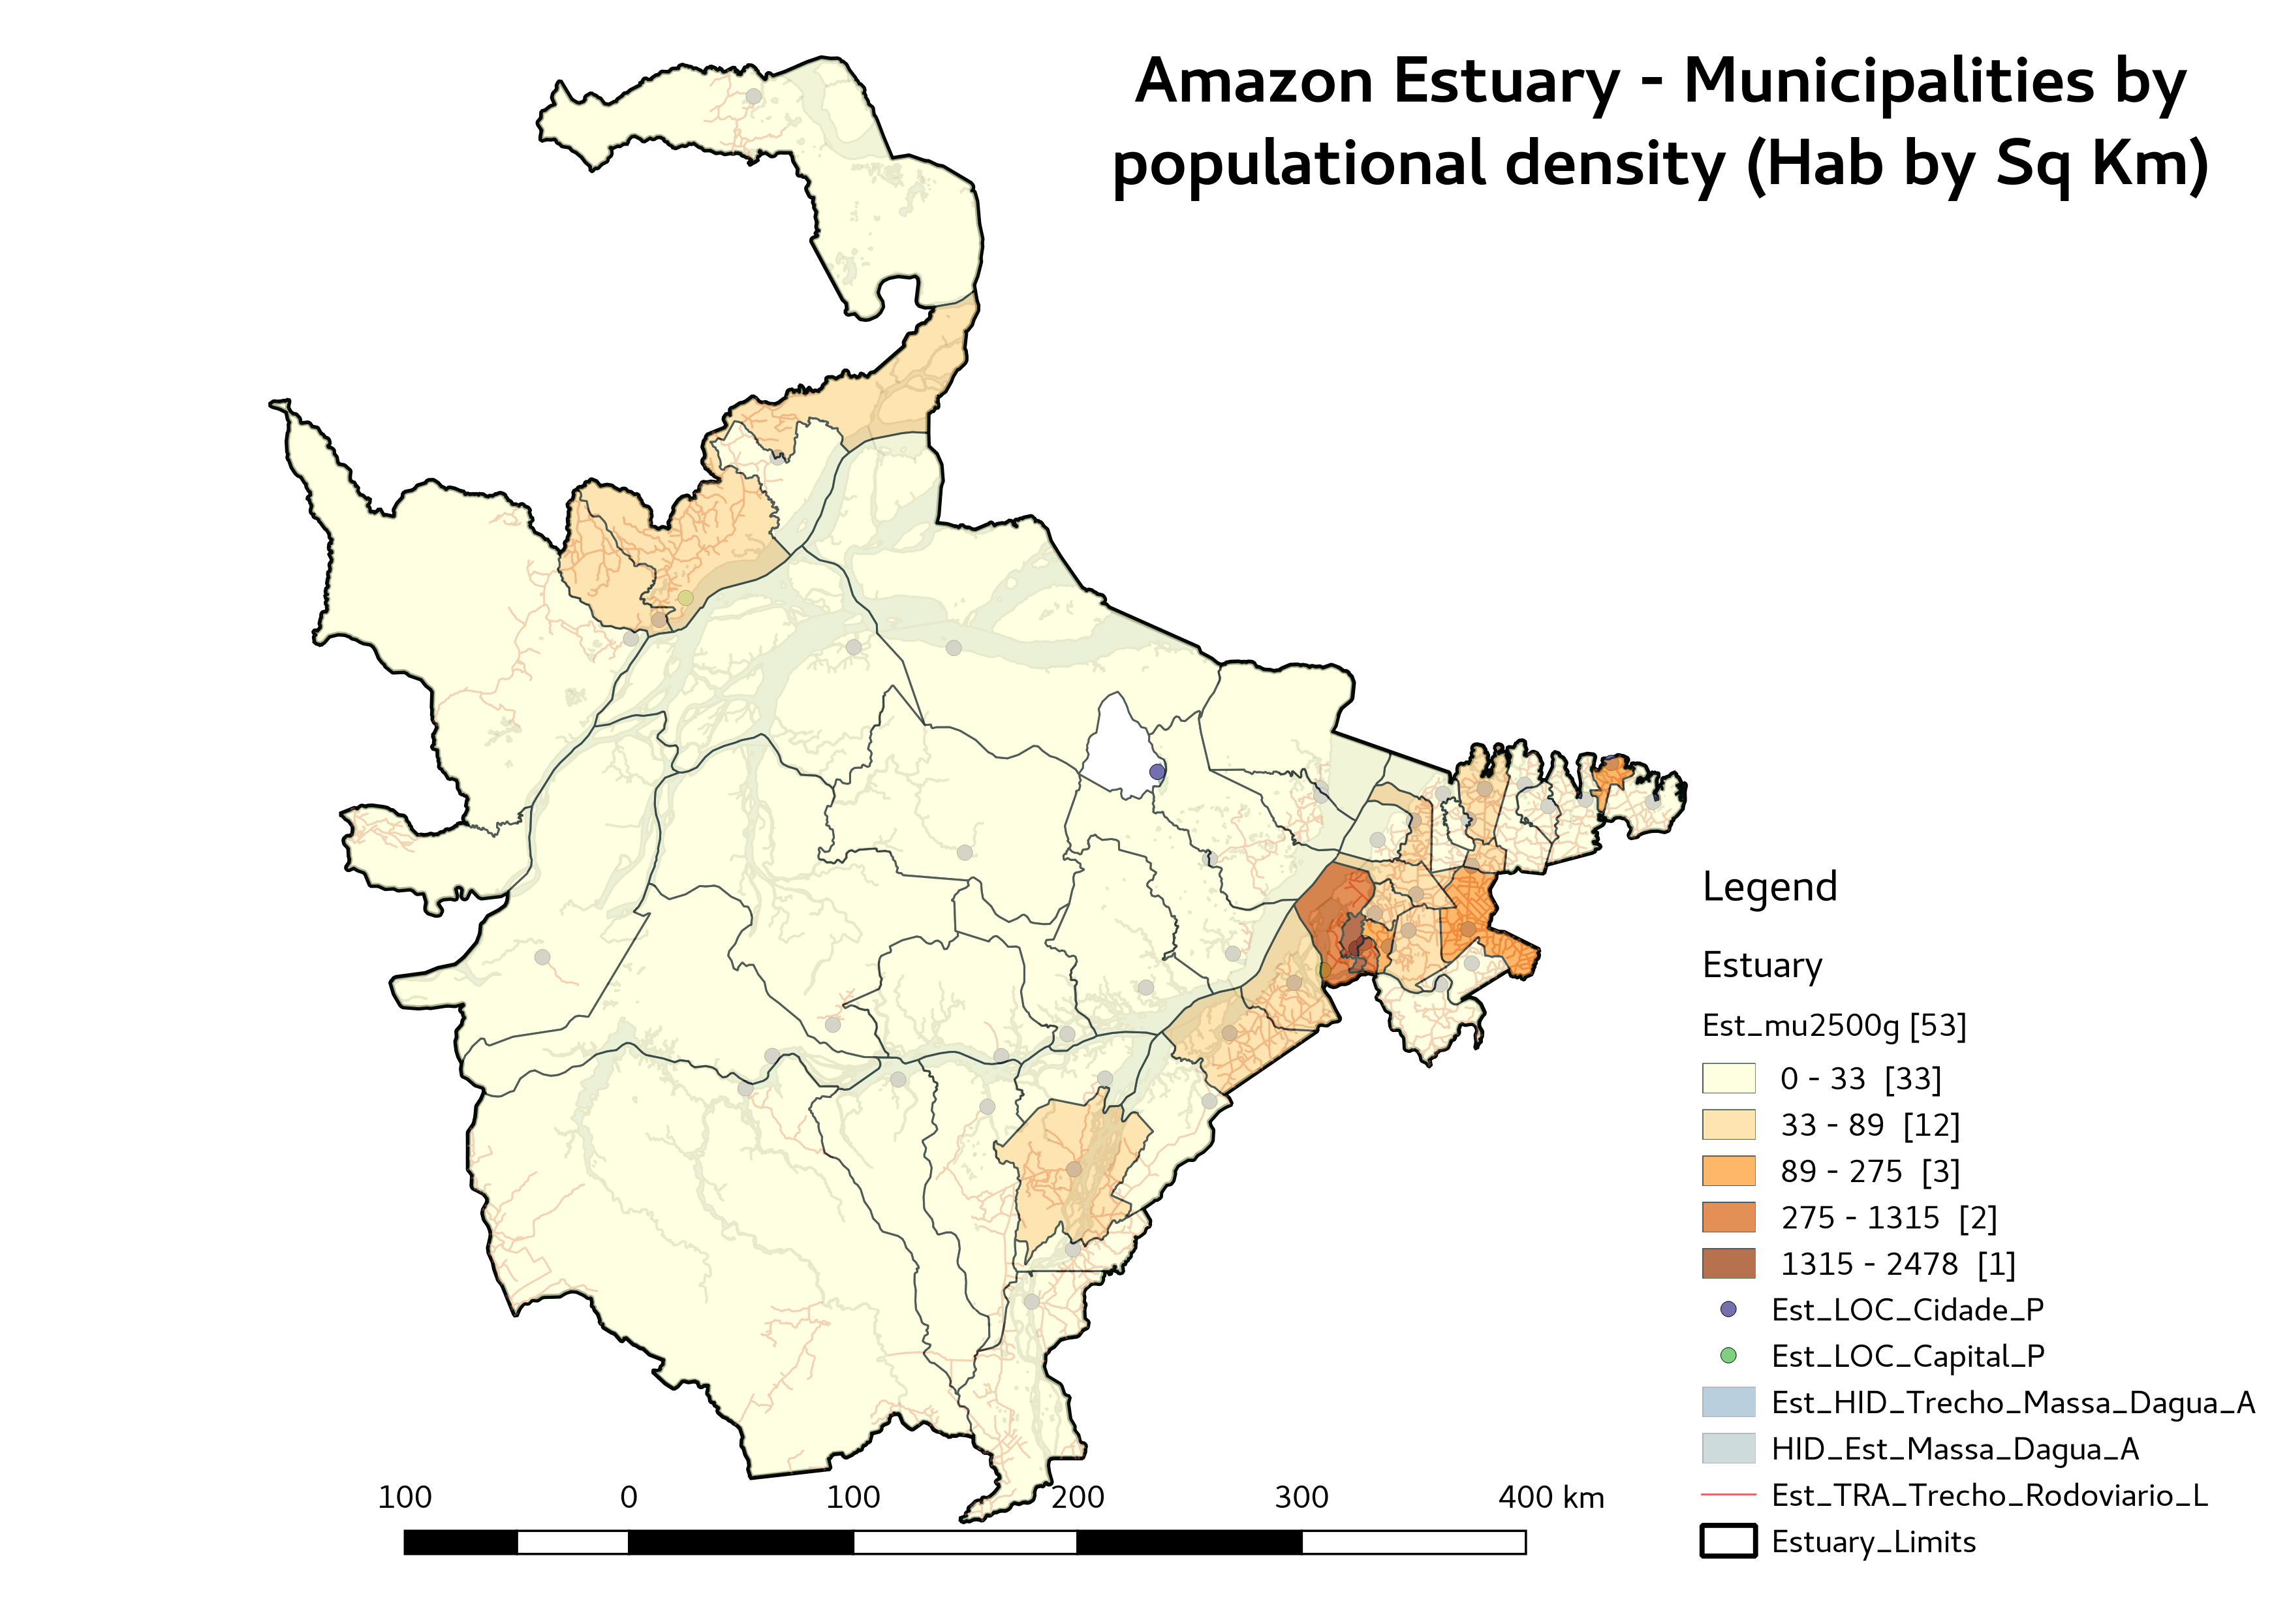
\includegraphics[width=\linewidth]{../figs/Estuary_PopDensity}
	\caption{Densidade Populacional no Estuário}
	\label{fig:estuarypopdensity}
\end{figure}
  
\lipsum[12-13]
  
\begin{table}[htbp]
\centering
	\caption{População Urbana e Rural das PeCiDAm}
	\begin{tabular}{l|rrrrr}
		\hline
		& \multicolumn{1}{c}{1970} & \multicolumn{1}{c}{1980} & \multicolumn{1}{c}{1991} & \multicolumn{1}{c}{2000} & \multicolumn{1}{c}{2010} \\ \hline
		Abaetetuba U & 19.785 & 33.748 & 56.389 & 70.843 & 82.998 \\ 
		Abaetetuba R & 37.735 & 40.793 & 43.600 & 48.309 & 58.102 \\ \hline
		Ponta U & 2.003 & 2.908 & 5.866 & 8.641 & 12.424 \\ 
		Ponta R & 8.995 & 9.966 & 10.634 & 10.053 & 13.575 \\ \hline
		Mazagao U & 1.675 & 2.517 & 3.921 & 5.972 & 8.272 \\ 
		Mazagao R & 8.822 & 17.916 & 4.990 & 6.014 & 8.760 \\ \hline
		Santana U & \multicolumn{1}{l}{...} & \multicolumn{1}{l}{...} & 45.800 & 75.849 & 99.111 \\ 
		Santana R & \multicolumn{1}{l}{...} & \multicolumn{1}{l}{...} & 5.651 & 4.590 & 2.151 \\ \hline
		\end{tabular}\\
		Fonte: IBGE – Censos Demográficos 
		\label{tab:popURPeCiDAm}
\end{table}

 \lipsum[12-13]



\chapter{Resultados}

  \lipsum[12-18]

\chapter{Conclusões}

  \lipsum[12-16]
  
  
  

%\bibliographystyle{unsrt}
\bibliographystyle{alpha}
\bibliography{../bib/bibliografia}

%\appendix

%\chapter{Tabelas demográficas}

%\lipsum[12-16]

%\begin{equation}
%  \label{eq:C}
%  \frac{\partial H}{\partial x} = -X
%\end{equation}

%\chapter{PeCiDAm}

%\lipsum[16-22]




\end{document}
